\section{Intel Movidius Neural Compute Stick}
\label{sec:movidius}
Today, low-power consumption is indispensable for unmanned vehicles and 
IoT\footnote{Internet of Things} devices.
In order to develop deep learning inference application at the edge, we can use 
Intel’s both energy efficient and low cost Movidius 
USB\footnote{Universal Serial Bus} stick (figure \ref{fig:movidius}).
Movidius Neural Compute Stick (NCS) is produced by Intel and can be run 
without any need of Intenet. 
This software development kit enables rapid prototyping, validation, and 
deployment of deep neural networks. 
Profiling, tuning, and compiling a DNN on a development computer is possible 
with the tools provided by the Intel Movidius Neural Compute SDK.
The Movidius NCS’ compute capability comes from Myriad 2 VPU\footnote{Vision Processing Unit}.
Intel Movidius VPUs drive the demanding workloads of modern computer vision 
and AI applications at ultra-low power. 
By coupling highly parallel programmable compute with workload-specific hardware 
acceleration, and co-locating these components on a common intelligent memory 
fabric, Movidius achieves a unique balance of power efficiency and high performance. 
Movidius technology allows device makers to deploy deep neural network and 
computer vision applications in categories such as smart-phones, drones, 
intelligent cameras and augmented reality devices.
Running Deep Learning models efficiently on low capacity graph processors is 
very painful. 
Movidius allows us to optimize the operation of large models such as GoogLeNet.
with multi-use support.
It is an easy-to-use kit that allows you to design and implement applications 
such as classification and object recognition as physical products.
We can simply think of Movidius NCS as a GPU\footnote{Graphics Processing Unit} 
running on USB. 
However, training of the model is not performed on this unit, the trained model 
works optimally on the unit and is intended to be used in physical environments 
for testing purposes.
%
\begin{figure}[htb]
\centering
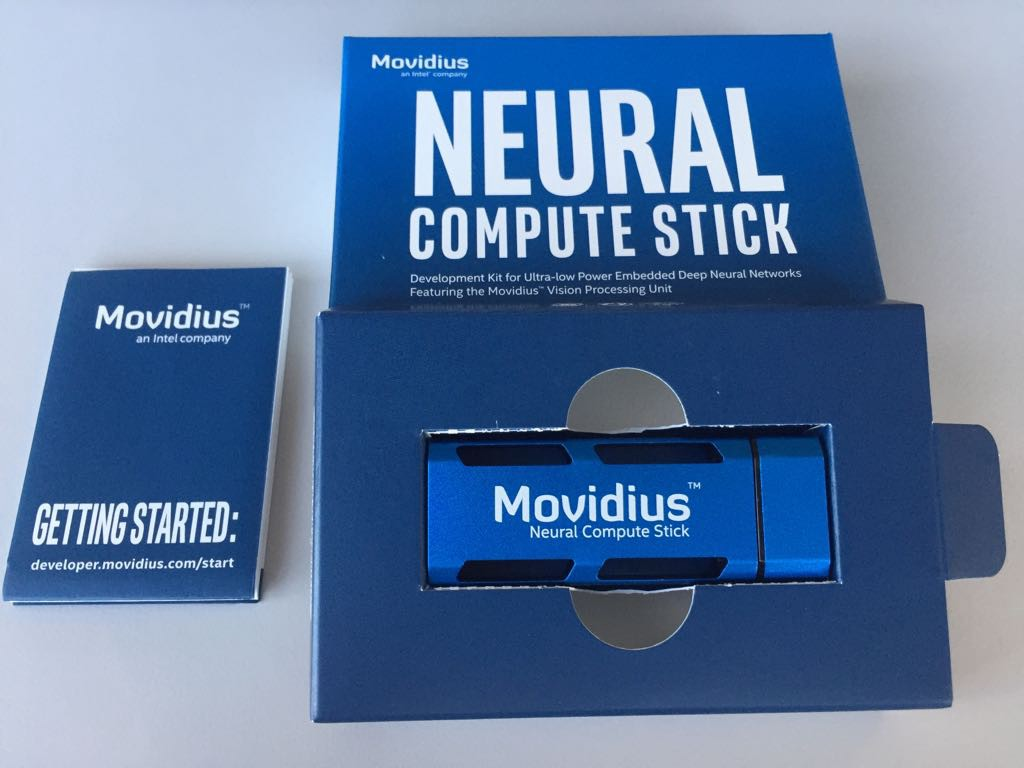
\includegraphics[width=\linewidth]{movidius}
\caption{Intel Movidius in package}
\label{fig:movidius}
\end{figure}
%
\subsection{Inside Intel Movidius}
\label{subsec:techspec}
Movidius provides the ultimate in low-power vision processing solutions, which 
include the Myriad 2 family of vision processing units (VPUs) plus a 
comprehensive Myriad Development Kit, a reference hardware EVM and 
optional Machine Vision Application Packages.
The Myriad 2 MA2x5x family of system-on-a-chip (SoC)\footnote{System on Chip} 
devices offers significant computation performance and image processing 
capability with a low-power footprint.
The Myriad 2 line up includes the following product configurations:
\begin{itemize}
	\item	MA2150: 1 Gbit DDR
	\item	MA2155: 1 Gbit DDR and secure boot 
	\item	MA2450: 4 Gbit DDR
	\item	MA2455: 4 Gbit DDR and secure boot
\end{itemize}
%
\begin{figure}[!h]
\centering
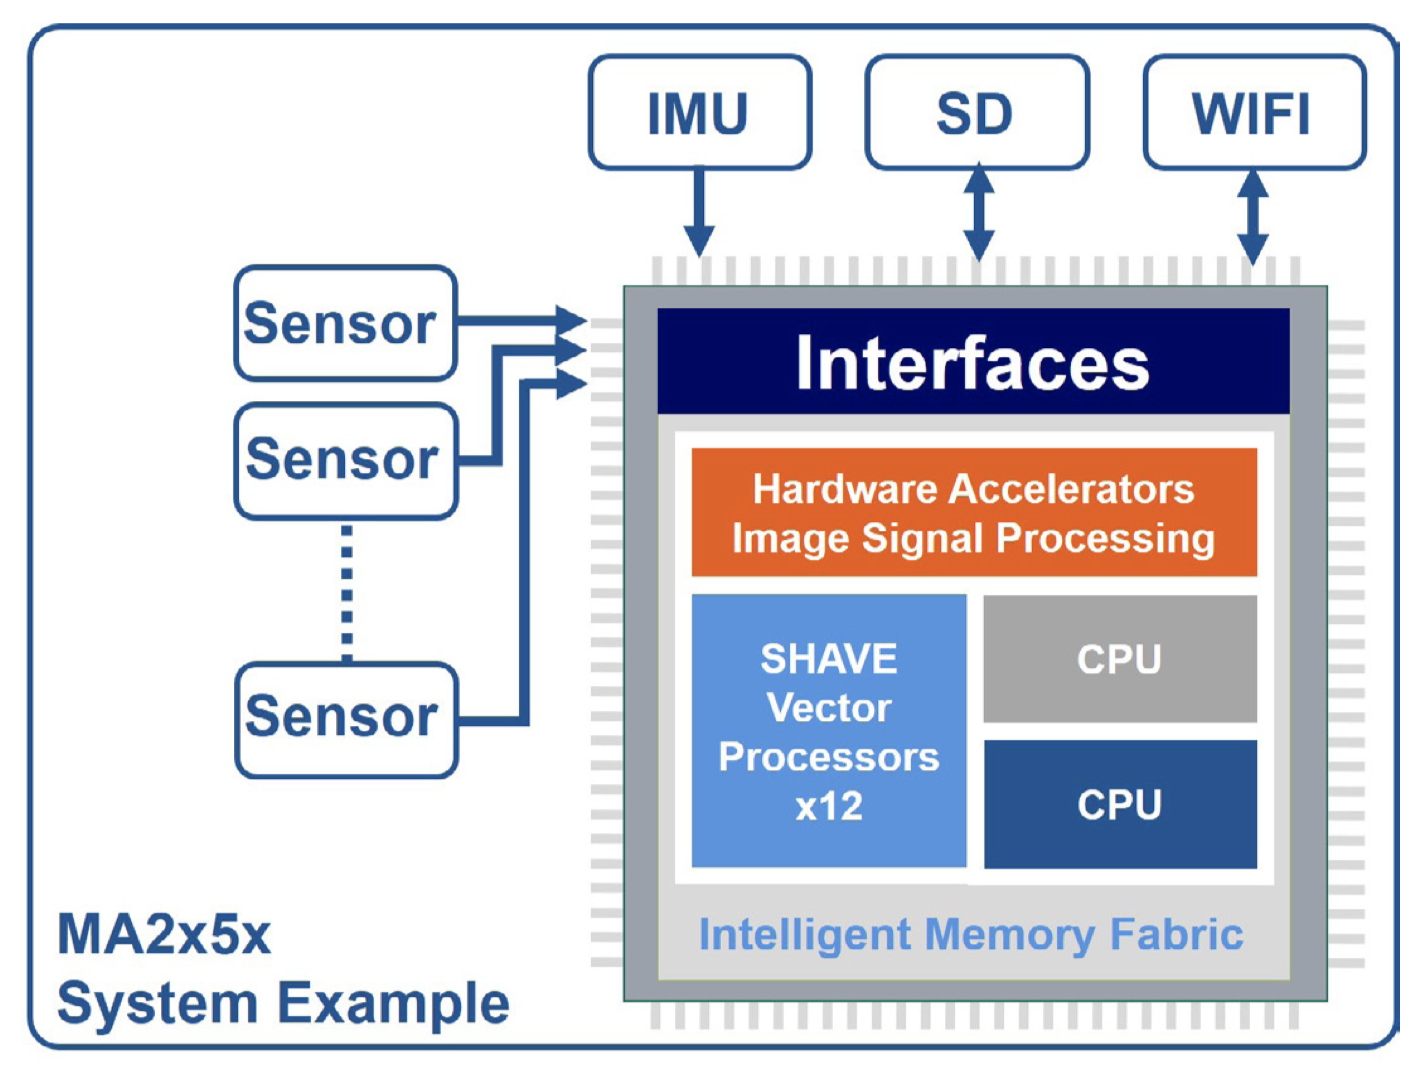
\includegraphics[width=0.65\linewidth]{system}
\caption{System example}
\label{fig:systemexample}
\end{figure}
% 
Myriad 2 VPUs offer TeraFLOPS (trillions of floating-point operations per 
second) of performance within a nominal 1 Watt power envelope. 
The Myriad 2 architecture, show in figure \ref{fig:architecture}, includes enough 
performance to support multiple cameras with flexible image signal processing 
pipelines for each camera, and software programmable vision processing with 
fixed- and floating-point data-types supported. 
A robust overall data-flow design ensures mitigation of processing bottlenecks.\\
Myriad 2 MA2x5x incorporates an innovative approach to combine image signal 
processing with vision processing. 
A set of imaging/vision hardware accelerators supports a world-class ISP pipeline 
without any round trips to memory; at the same time they are re-purposed to 
accelerate developers' vision processing algorithms in conjunction with a set of 
special purpose VLIW vision processor cores. 
All processing elements are tied together with a multi-ported memory that enables 
implementation of demanding applications with high efficiency.\cite{intel}\\
MYRIAD 2 SoC SPECIFICATIONS
\begin{itemize}
	\item Heterogeneous, high throughput, multi-core architecture based on:
	\begin{itemize}
		\item 12 VLIW 128-bit vector SHAVE Processors optimized for machine vision
		\item Configurable hardware accelerators for image and vision processing, with line-buffers enabling zero local memory access ISP mode
		\item 2 x 32-bit RISC processors 
		\item Supports data and task parallelism 
		\item Programmable Interconnect
		\end{itemize}
		\item Support for 16/32-bit floating point and 8/16/32-bit integer operations
		\item Homogeneous, centralized memory architecture
		\item 2MB of on-chip memory
		\item 400 GB/sec of sustained internal memory bandwidth
		\item 256 KB of L2 Cache
		\item Power management: 20 power islands; low power states
		\item Nominal 600 MHz operation at 0.9 V
		\item Rich set of interfaces:
		\begin{itemize}
			\item 12 Lanes MIPI, 1.5 Gbps per lane configurable as CSI-2 or DSI
			\item I2C, SPI for control and configuration
			\item I2S for audio input
			\item Banks of configurable GPIO, PWM
			\item USB3 with integrated PHY
			\item 2-Slot SDIO
			\item Debug interface
			\item 1 Gbit Ethernet
		\end{itemize}
		\item Available package configurations:
		\begin{itemize}
			\item MA2150/MA2155: 6.5mm x 6.5mm 0.4mm pitch, 225 Ball BGA 1Gb LPDDR II
			\item MA2450/MA2455: 8mm x 9.5mm 0.5mm pitch, 270 Ball BGA, 4Gb LPDDR III
		\end{itemize}
		\item Advanced low-power 28nm HPC process node
\end{itemize}
%
\begin{figure}[htb]
\centering
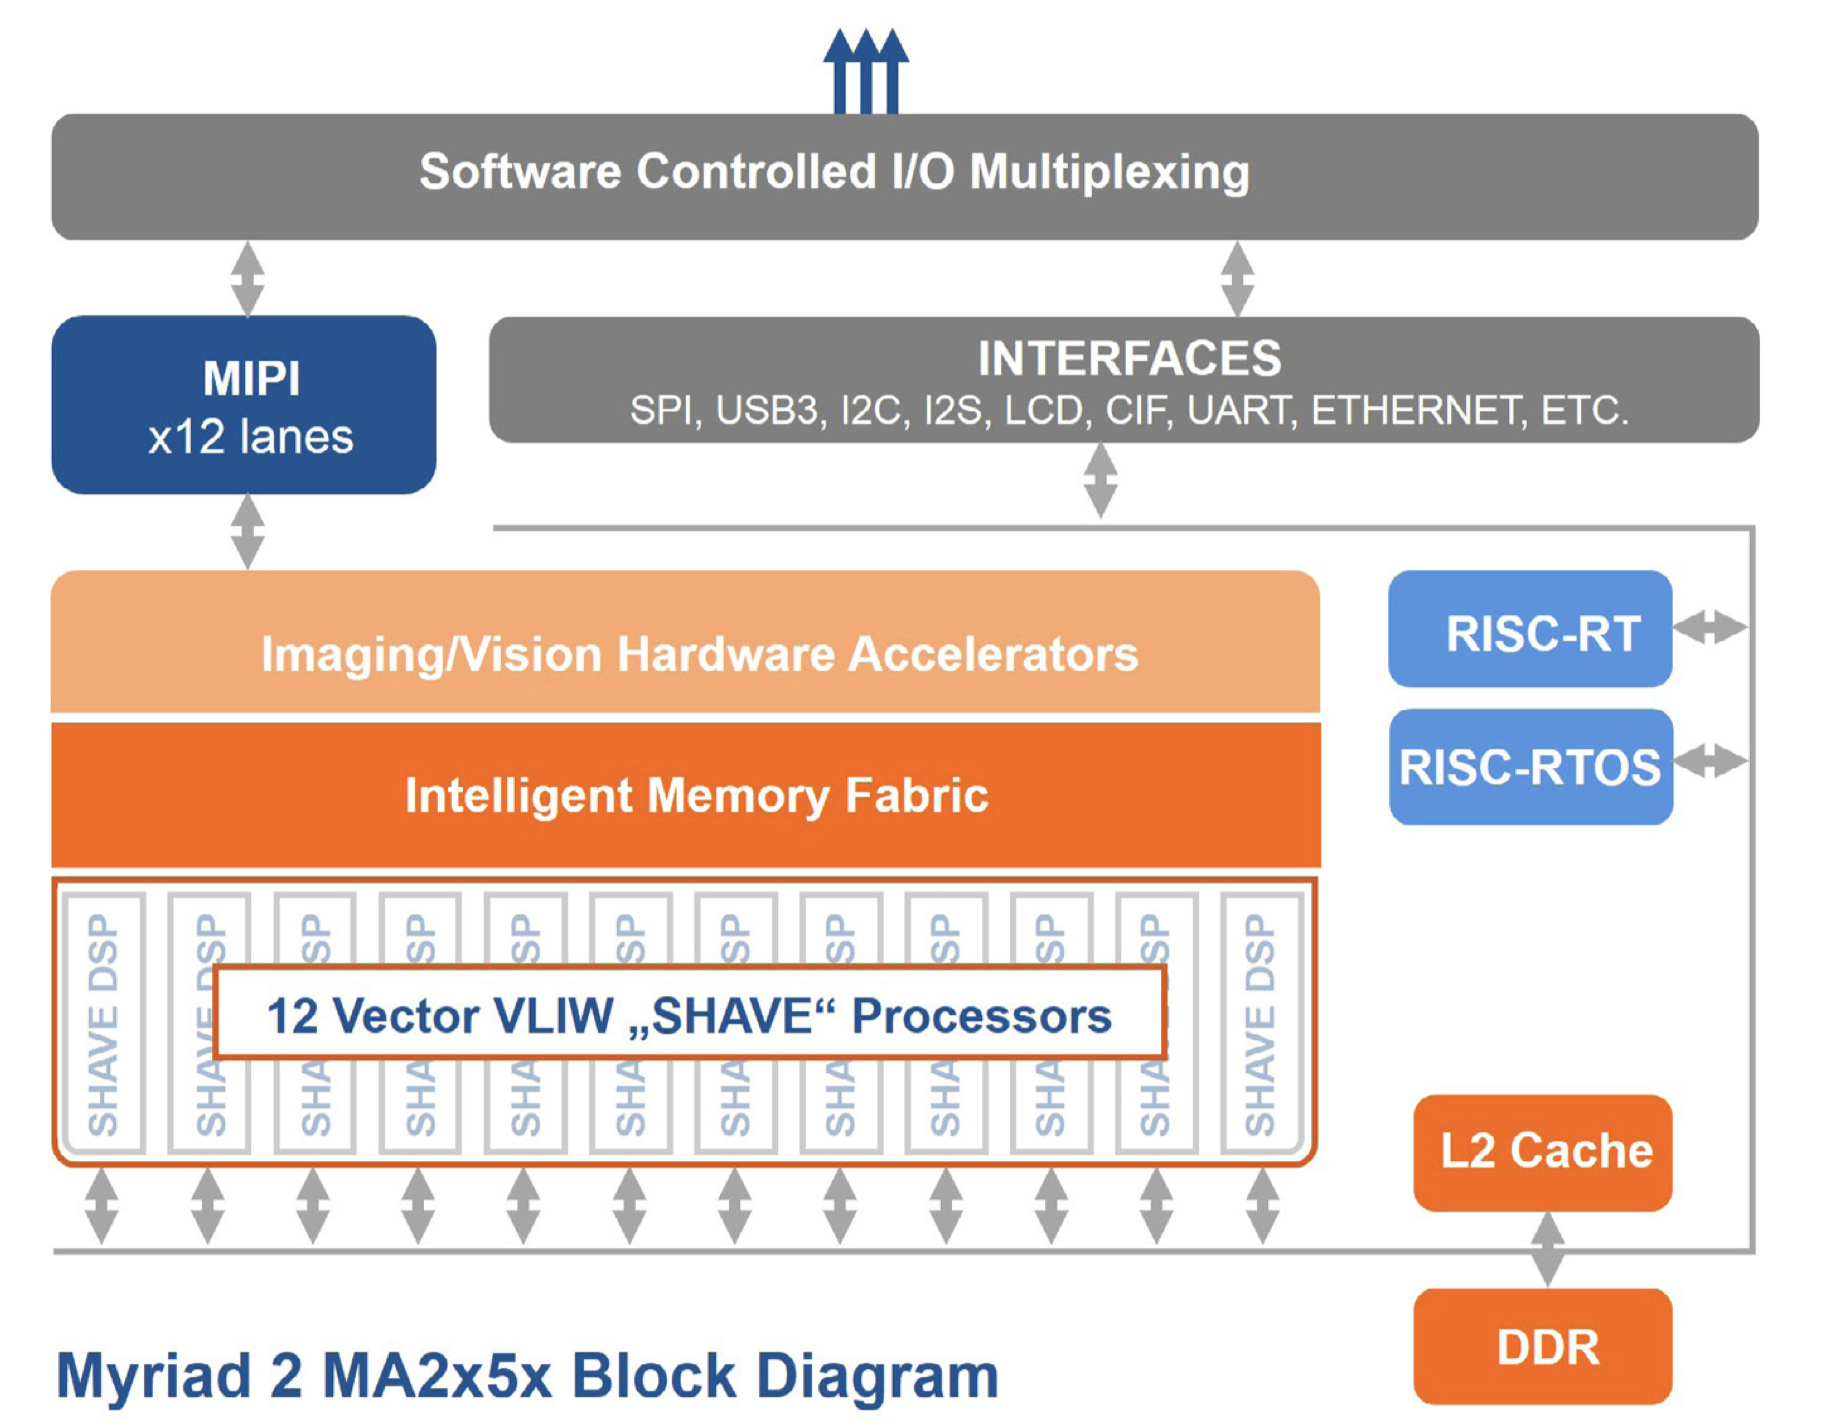
\includegraphics[width=\linewidth]{core}
\caption{MYRIAD 2 SoC architecture}
\label{fig:architecture}
\end{figure}
%
\subsection{Conversion}
\label{subsection:conversion}
Once the neural network training is complete, the file containing the 
definitions and weights of the various levels must be converted into a format 
that can be read by the Movidius device.
The Intel Movidius Neural Compute SDK enables rapid prototyping and deployment 
of deep neural networks (DNNs) on compatible neural compute devices like the 
Intel Movidius Neural Compute Stick. 
The NCSDK includes a set of software tools to compile, profile, and check 
(validate) DNNs as well as the Intel® Movidius™ Neural Compute API (Intel 
Movidius NCAPI) for application development in C/C++ or Python.
The NCSDK has two general usages:
Profiling, tuning, and compiling a DNN model on a development computer 
(host system) with the tools provided in the NCSDK.
Prototyping a user application on a development computer (host system), 
which accesses the neural compute device hardware to accelerate DNN inferences 
using the NCAPI. 
In fact, the tool made available by Intel allows to compile the file obtained; 
simply invoking the following expression from the command line:
%
\code{\$ mvNCCompile inception-v1.meta -s 12 -in=input -on=predictions/Softmax -is 224 224 -o InceptionV1.graph}
%
You can see that in the expression following the command there are some 
arguments, let's examine them:
\begin{itemize}
\item \textbf{*.pb} the trained network file.
\item \textbf{[-s max\_number\_of\_shaves]} Specify the maximum number of SHAVEs 
to use for network layers (default: 1).
The number of available SHAVEs depends on your neural compute device; refer to 
figure \ref{fig:architecture}
\item \textbf{[-in input\_node\_name]} This option is required for TensorFlow 
networks. 
You can use the name parameter (available for most layers) when creating your 
network and pass that name into this option.
\item \textbf{[-on output\_node\_name]} Specify an alternative end point for the 
network. 
By default the network’s end point is the output layer. 
This option enables partial network processing. When used together with the 
-in option, the user can isolate one or more layers in a network for analysis.
\item \textbf{[-is input\_width input\_height]} Specify input dimensions for 
networks that do not have dimension constraints on the input layer.
This option assumes that the batch size is 1 and the number of channels is 3.
\item \textbf{[-o output\_graph\_filename]} Specify an output graph file-name. 
If this is not provided, \emph{``graph"} will be used for the file-name.
\end{itemize}

\subsection{Result}
\label{subsec:result}




